\chapter{Metodología y gestión del proyecto}
\label{chap:metodologia}
En este capítulo se aborda la metodología seguida para la realización del proyecto, explicando los principios fundamentales da la misma además de los motivos de su elección, junto con las adaptaciones que se consideraron necesarias en el contexto de este proyecto. Por otro lado, también se describe la planificación realizada para la consecución del proyecto incluyendo el análisis de riesgos realizado.

\section{Metodología}
La metodología constituye un aspecto esencial para garantizar que un proyecto se desarrolle de manera eficiente, produzca un producto de alta calidad y cumpla con los objetivos propuestos. Esta proporciona una estructura y un enfoque organizado que permite aumentar la productividad y evitar las desviaciones de estos. La elección de una metodología adecuada es crucial para el éxito del proyecto y debe adaptarse a las necesidades, características y contexto específicos tanto del proyecto como del equipo de trabajo.\\
En nuestro caso, existen varios factores dentro del proyecto que condicionan en gran medida la elección del enfoque metodológico:\\
\begin{itemize}
    \item El carácter altamente innovador de la propuesta del proyecto.
    \item La escasez relativa y falta de homogeneidad en los experimentos en técnicas de clasificación de texto, como perfilado automático, en idioma español en comparación con el inglés.
    \item El escaso conocimiento inicial del alumno acerca de estas técnicas y la relativa complejidad y novedad de los algoritmos de procesado de lenguaje actual.
    \item La falta de acotación y ambigüedad de los requisitos iniciales del producto propuesto.
\end{itemize}
% elección de una metodología debe considerar el entorno dinámico y desafiante en el que se desenvolverá el proyecto. En este escenario, las metodologías ágiles se destacan como una opción atractiva. Estas metodologías ofrecen la flexibilidad necesaria para adaptarse a los cambios, promover la colaboración activa en el equipo y permitir la entrega incremental de resultados.

% Dado el carácter altamente innovador de la propuesta del proyecto, las metodologías ágiles son ideales para abordar situaciones en las que los requisitos pueden evolucionar a medida que se adquiere un mejor entendimiento del dominio. Además, la escasez de experimentos en técnicas de clasificación de texto en español requiere un enfoque que permita la experimentación y la incorporación ágil de nuevos conocimientos.

% El conocimiento inicial limitado del alumno puede abordarse de manera efectiva con metodologías ágiles, ya que promueven el aprendizaje continuo y la adaptación a medida que se adquieren habilidades y experiencia. Por último, la falta de acotación en los requisitos iniciales se beneficia de la capacidad de las metodologías ágiles para gestionar la incertidumbre y permitir cambios en el alcance del proyecto.

% En resumen, dadas las condiciones y desafíos particulares de este proyecto, la elección de una metodología ágil proporciona la agilidad, adaptabilidad y enfoque en la colaboración necesarios para alcanzar el éxito en un entorno altamente innovador y dinámico. Esta elección metodológica permitirá abordar los desafíos y cambios que surjan en el camino y garantizar que el proyecto se desarrolle de manera efectiva y cumpla con sus objetivos.
Teniendo estos factores en cuenta, las metodologías ágiles se destacan como una opción atractiva. Estas metodologías ofrecen la flexibilidad necesaria para adaptarse a cambios en los requisitos a medida que se adquiere un mejor conocimiento del dominio, promueve el aprendizaje continuo dentro de un entorno complejo y permiten la entrega incremental de resultados. Dentro de las opciones disponibles dentro de este grupo de metodologías se ha optado por Scrum (\cite{scrum}) por ser una de las de mayor relevancia y conocimiento en el sector TIC actual.\\
\subsection{Scrum}
Scrum es un marco de trabajo ágil ampliamente utilizado en el desarrollo de software y en la gestión de proyectos. Fue creado para abordar los desafíos de proyectos complejos y cambiantes, permitiendo la entrega de productos con el máximo valor posible optimizando la creatividad y productividad en el proceso. En la figura \ref{fig:scrum} se puede ver un diagrama explicativo donde se muestra el proceso de Scrum.\\
\noindent\begin{figure}[hp!]
  \centering
    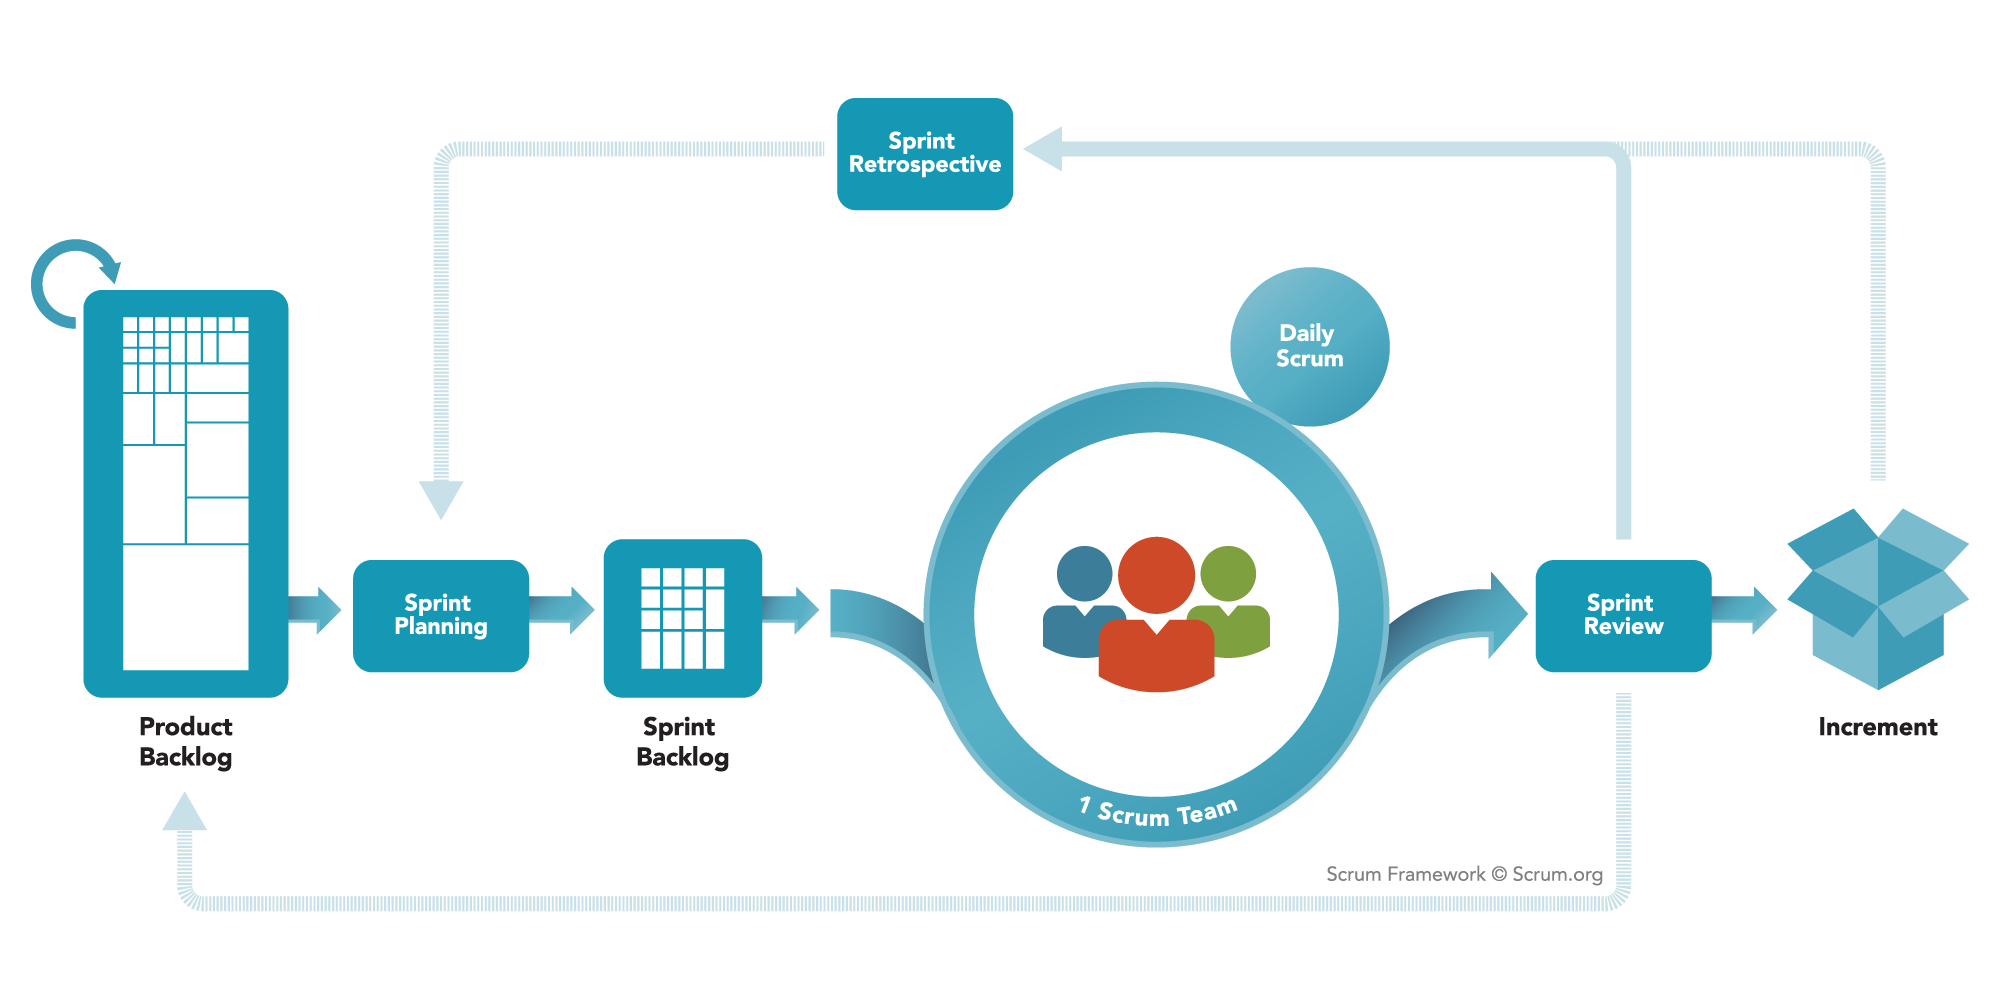
\includegraphics[width=\textwidth]{imaxes/scrum.png}
  \caption{Diagrama de la metodología \textit{Scrum}.}
  \label{fig:scrum}
\end{figure}
Scrum se basa en la teoría del control empírico de procesos, o empirismo. Esta sostiene que el conocimiento proviene de la experiencia y de tomar decisiones basadas en lo que se sabe. Este marco de trabajo propone un enfoque iterativo e incremental para mejorar la predictibilidad y controlar el riesgo. Tres pilares respaldan cada implementación del control empírico de procesos: transparencia, inspección y adaptación.
\begin{itemize}
    \item \textbf{Transparencia}: Aspectos significativos del proceso deben ser visibles para quienes son responsables del resultado. La transparencia requiere que esos aspectos estén definidos por unos estándares comunes para que los responsables tengan un entendimiento acorde acerca de estos resultados.
    \item \textbf{Inspección}: Los usuarios de Scrum deben revisar con frecuencia los artefactos de Scrum y el progreso hacia un objetivo común para detectar desviaciones no deseadas.
    \item \textbf{Adaptación}: Si durante la inspección del trabajo un miembro del equipo determina que ha habido desviaciones significativas con respecto a los objetivos iniciales el proceso y las tareas deben adaptarse lo antes posible con el objetivo de reducir o eliminar esta desviación.
\end{itemize}
\subsubsection{Roles}
Un equipo de Scrum debe ser auto-organizativo y multifuncional: el equipo debe ser capaz de dirigirse a sí mismo y debe poseer las competencias necesarias para la consecución del trabajo sin dependencias externas. Para ello se definen los siguientes roles:
\begin{itemize}
    \item \textit{Product Owner}: este es responsable de maximizar el valor del producto resultado del trabajo del \textit{equipo de desarrollo}. La forma en que esto se consiga puede variar de un equipo a otro.
    \item \textit{Equipo de desarrollo}: este esta formado por profesionales que se encargan de la realización del producto <<Terminado>> después de cada incremento, el cual constituye los resultados del mismo.
    \item \textit{Scrum master}: este es responsable de promover y apoyar que se siguen las pautas correctas de realización del Scrum en el proyecto. Debe ayudar a que el equipo entienda los conceptos de scrum para poder maximizar el valor entregado.
\end{itemize}
\subsubsection{Eventos}
Además de los roles anteriores existen una serie de eventos pre-establecidos con una duración predeterminada. Estos tienen como finalidad la establecer una regularidad en el proyecto de forma que se minimicen las reuniones no establecidas por scrum. Estos eventos son:
\begin{itemize}
    \item \textit{Sprint}: constituye un incremento o iteración del producto. Tiene una duración generalmente de entre 2-4 semanas en el que se desarrolla una parte del producto. Durante el sprint, el equipo se compromete a entregar un conjunto específico de funcionalidades.
    \item \textit{Sprint planning}: la planificación del sprint es una reunión entre el todos los miembros del equipo, donde se define de forma colaborativa el trabajo que se llevará a cabo durante el mismo. Tiene una reunión máxima de ocho horas, aunque suele ser menor según la duración del sprint.
    \item \textit{Daily scrum}: se trata de una breve reunión (máximo 15 minutos) donde el equipo de trabajo planifica las tareas que se llevarán a cabo durante el día. Además, se realiza una inspección para verificar que el equipo progrese adecuadamente hacia los objetivos marcados.
    \item \textit{Sprint review}: esta reunión de carácter más informal se da al final de cada sprint. En ella el equipo completo (junto a \textit{stakeholders}\footnote{Aquellos interesados en la realización del proyecto.}) realiza la inspección del incremento demostrando los resultados del sprint y añadiendo al \textit{product backlog} aquellas funcionalidades <<terminadas>>.
    \item \textit{Sprint retrospective}: reunión de carácter más filosófico que se da entre el \textit{Sprint review} y el próximo \textit{Srint planning} donde el equipo <<se inspecciona a sí mismo>>: se comparten impresiones acerca del incremento, reflexionando acerca de aquellos aspectos del proceso que han ido bien y aquellos que son sujetos de mejora.

\end{itemize}
\subsubsection{Artefactos}
Los artefactos de Scrum representan valor o trabajo diseñados para mejorar la transparencia y facilitar la inspección del proyecto. Esto artefactos son los siguientes:
\begin{itemize}
    \item \textit{Product backlog}: esta es una lista ordenada de todas aquellas funcionalidades y tareas que serán necesarias en el producto. Este representa los requisitos deseado del producto. Esta nunca está del todo completa: evoluciona a lo largo del tiempo con el producto a medida que los requisitos cambian o se entienden mejor.
    \item \textit{Sprint backlog}: conforma el conjunto de elementos del \textit{Product backlog} escogidos para su realización en el marco de un \textit{Sprint}. Este incluye el plan diseñado para la entrega de incremento en cuestión y la realización del objetivo del mismo.
\end{itemize}
\subsection{Adaptaciones de \textit{Scrum} al proyecto}
Varios factores como la presencia de un único miembro en el equipo de desarrollo, la falta de regularidad en la dedicación del mismo debido a obligaciones académicas han impedido que se haya podido llevar a cabo la metodología seleccionada de forma totalmente fiel a sus pautas. Por un lado se ha realizado la siguiente asignación de roles:

\begin{itemize}
    \item El rol de \textit{Product owner} ha sido desempeñado por %el alumno Nicolás Míguez García
    \item El rol de \textit{Scrum master} ha sido desempeñado por %los directores de este proyecto Patricia Martín Rodilla y David Otero Freijeiro..
    \item El de equipo de trabajo estuvo constituido por un único miembro, el alumno Nicolás Míguez García.
\end{itemize}
A continuación, se presentan las modificaciones implementadas en la metodología original para adecuarla a las necesidades de este proyecto:
\begin{itemize}
    \item La duración de cada \textit{sprint} ha ido variando (entre 3 y 5 semanas).
    \item De la misma forma que la duración, la carga de trabajo en cada sprint ha ido variando, en función de la dedicación disponible por parte del equipo de desarrollo.
    \item Dado que el equipo de desarrollo está compuesto por una sola persona, el evento de \textit{Daily scrum} pierde el sentido de su existencia. Sin embargo, se mantiene la práctica de la revisión del trabajo diario como parte de las responsabilidades del alumno.
\end{itemize}
\subsubsection{Historias de usuario}
Para definir los elementos del \textit{Product backlog} (y por tanto los requisitos funcionales del proyecto) se han usado las historias de usuario. Estas constituyen una técnica muy utilizada en metodologías ágiles para la especificación de requisitos debido a su sencillez y claridad. Estas se tratan descripciones breves (una o dos líneas) de las funciones del sistema desde la perspectiva del usuario. Las historias de usuario tienen de la siguiente forma:
\begin{center}
     \textit{Como <rol> quiero <algo> para poder <beneficio>.}
\end{center}
%Para medir el esfuerzo necesario para completar una historia de usuario, se emplean puntos de historia. Estos puntos reflejan el nivel de esfuerzo teniendo en cuenta varios factores, como la cantidad de trabajo, la complejidad del mismo o el riesgo asociado.

Por otro lado, debido a que la primera fase del proyecto estaba más orientada hacia la investigación y desarrollo de los algoritmos de perfilado automático que al desarrollo de un producto software en sí mismo, el modelado de requisitos desde la perspectiva de usuario no tiene demasiado sentido. Es por ello que los requisitos de esta fase se modelan como tareas técnicas orientadas al desarrollador en vez de al usuario.% No obstante, por ser uniformes en todo el proyecto el esfuerzo en estas tareas técnicas se modelará igualmente mediante puntos de historia.

\section{Gestión del proyecto}
La gestión del proyecto se encarga de la planificación, seguimiento y control del mismo, teniendo en cuenta factores como la estimación, la asignación y control de recursos, y la gestión de riesgos. Esto proporciona una visión global acerca del estado del proyecto en cualquier momento de su desarrollo.
\subsection{Recursos}
\subsection{Planificación}
\subsection{Gestión de riesgos}
